
\chapter{Celestial Phenomena}

\begin{figure}[h]
   \vspace{-40pt}
   \centering
   %\vspace*{\fill}
   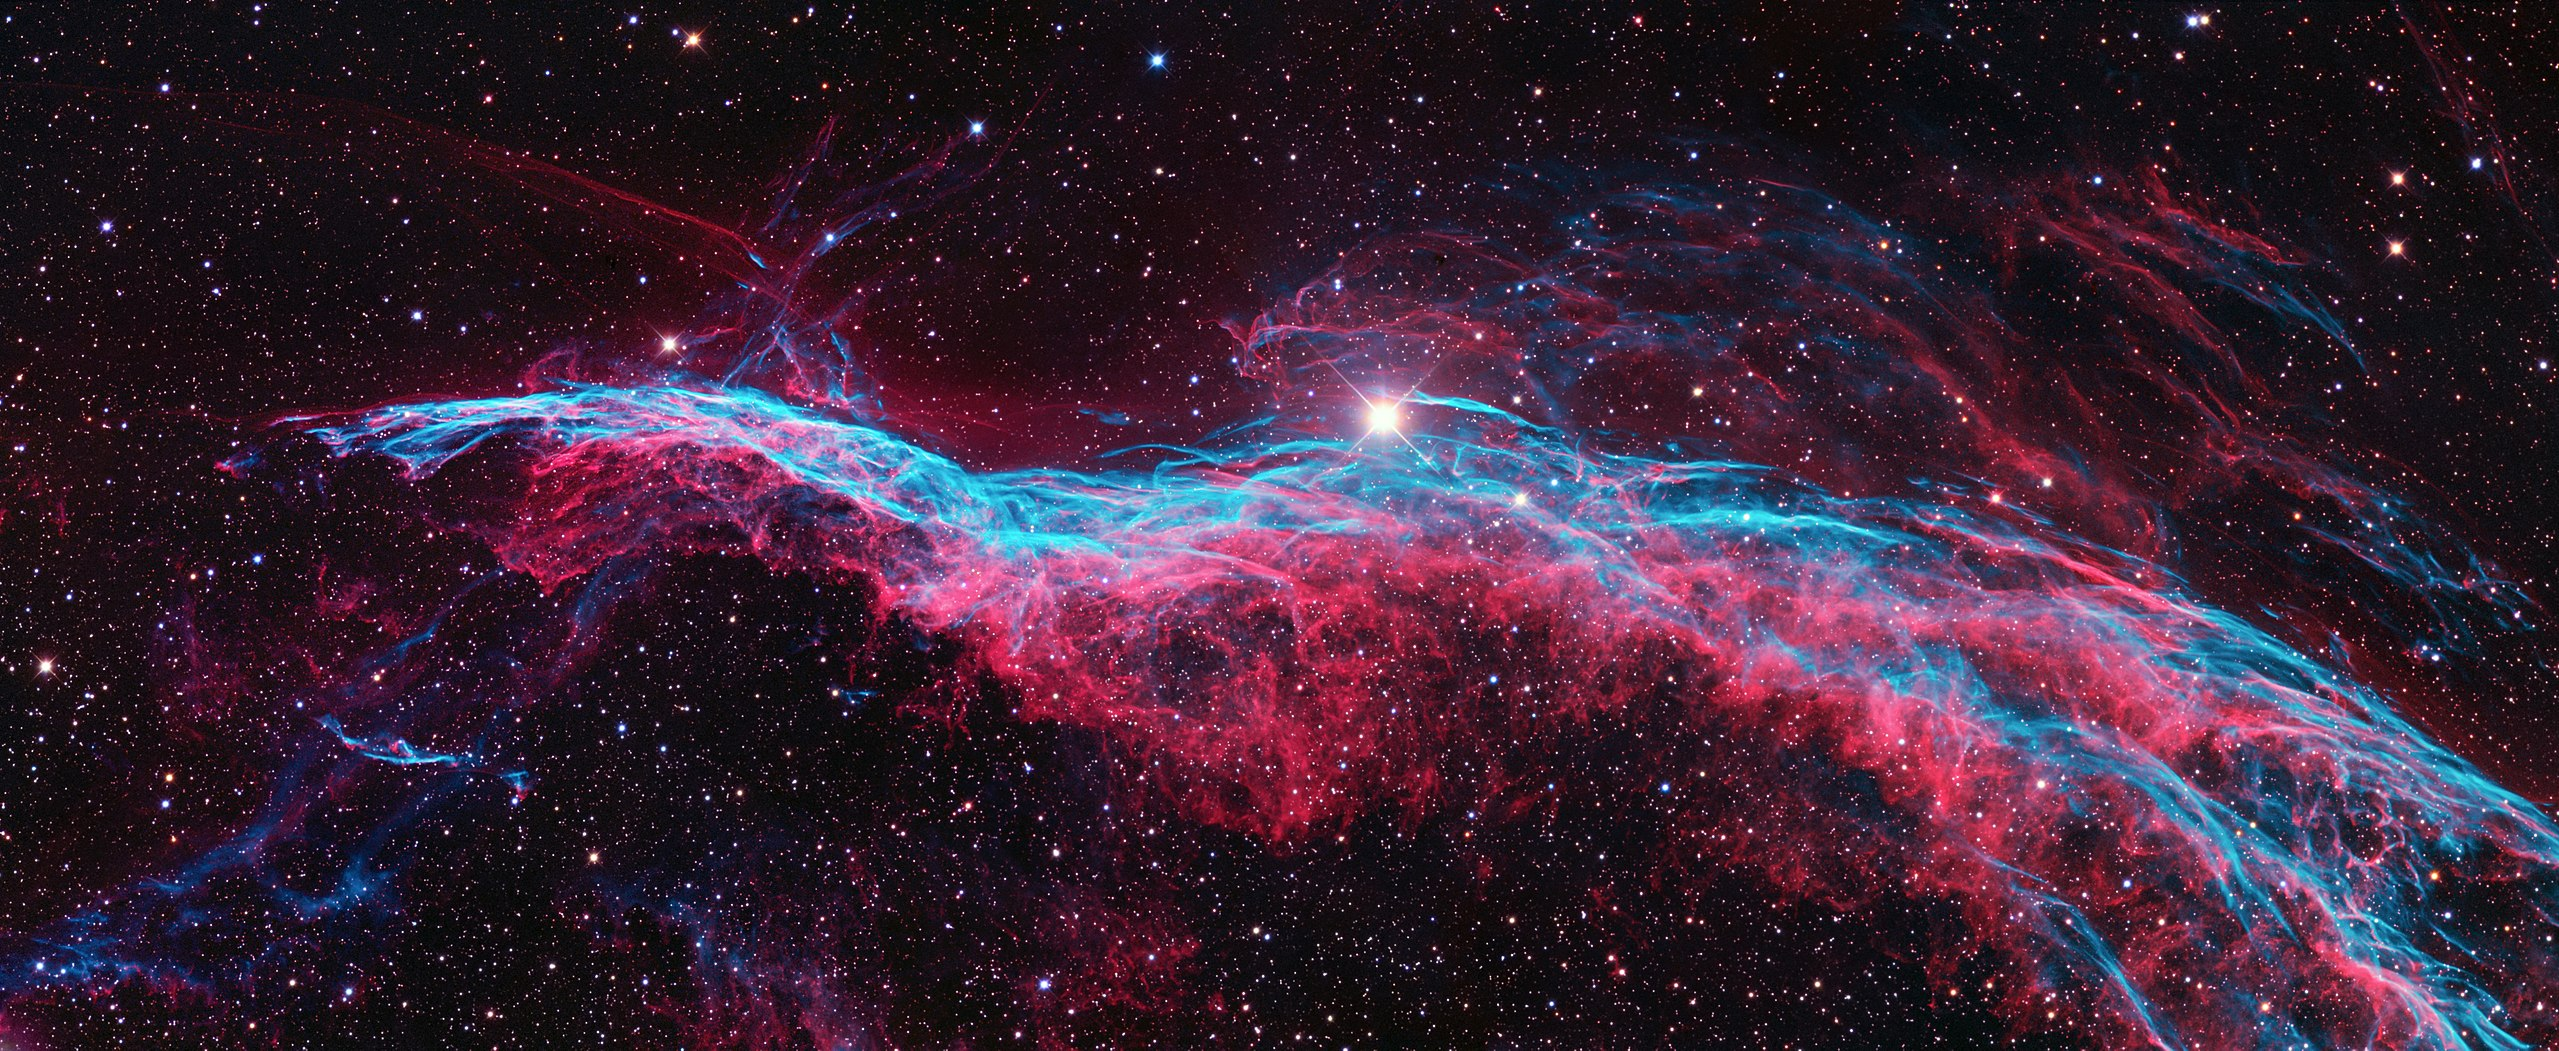
\includegraphics[width=\linewidth]{../../pictures/2560px-Veil_Nebula_-_NGC6960.jpg}
   \captionsetup{width = \linewidth}
   \caption{\footnotesize Image of the Veil Nebula. Author: \href{https://commons.wikimedia.org/wiki/File:Veil_Nebula_-_NGC6960.jpg}{Ken Crawford}.
      License: \href{https://creativecommons.org/licenses/by-sa/3.0/deed.en}{CC BY-SA 3.0}
   }
   \vspace*{\fill}
\end{figure}
\clearpage

\lettrine[lines=4]{\goudy A}{nother} course of ideas must, however, be pursued in a work which proposes merely to give an exposition of what is known, of what may in the present state of our knowledge be regarded as certain, or as merely probable in a greater or lesser degree, and does not enter into a consideration of the proofs on which such results have been based. Here, therefore, we do not proceed from the subjective point of view of human interests. The terrestrial must be treated only as a part, subject to the whole. The view of nature ought to be grand and free, uninfluenced by motives of proximity, social sympathy, or relative utility. A physical cosmography - a picture of the universe - does not begin, therefore, with the terrestrial, but with that which fills the regions of space. But as the sphere of contemplation contracts in dimension, our perception of the richness of individual parts, the fullness of physical phenomena, and of the heterogeneous properties of matter becomes enlarged. From the regions in which we recognize only the dominion of the laws of attraction, we descend to our own planet, and to the intricate play of terrestrial forces. The method here described for the delineation of nature is opposed to that which must be pursued in establishing conclusive results. The one enumerates what the other demonstrates.

Man learns to know the external world through the organs of the senses. Phenomena of light proclaim the existence of matter in remotest space, and the eye is thus made the medium through which we may contemplate the universe. The discovery of telescopic vision more than two centuries ago has transmitted to the latest generations a power whose limits are as yet unattained. 

The first and most general consideration in the Cosmos is that of the contents of space -- the distribution of matter, or of creation, as we are wont to designate the assemblage of all that is and ever will be developed. We see matter either agglomerated into rotating, revolving spheres of different density and size, or scattered through space in the form of self-luminous vapor. If we consider first the cosmical vapor dispersed in definite nebulous spots, its state of aggregation will appear constantly to vary, sometimes appearing separated into round or elliptical disks, single or in pairs, occasionally connected by a thread of light; while, at another time, these nebul{\ae} occur in forms of larger dimensions, and are either elongated, or variously branched, or fan-shaped, or appear like well-defined rings, enclosing a dark interior. It is conjectured that these bodies are undergoing variously developed formative processes, as the cosmical vapor becomes condensed in conformity with the laws of attraction, either round one or more of the nuclei. Between two and three thousand of such unresolvable nebul{\ae}, in which the most powerful telescopes have hitherto been unable to distinguish the presence of stars, have been counted, and their positions determined.

\clearpage
\begin{wrapfigure}{r}{0.5\textwidth}
   \centering
   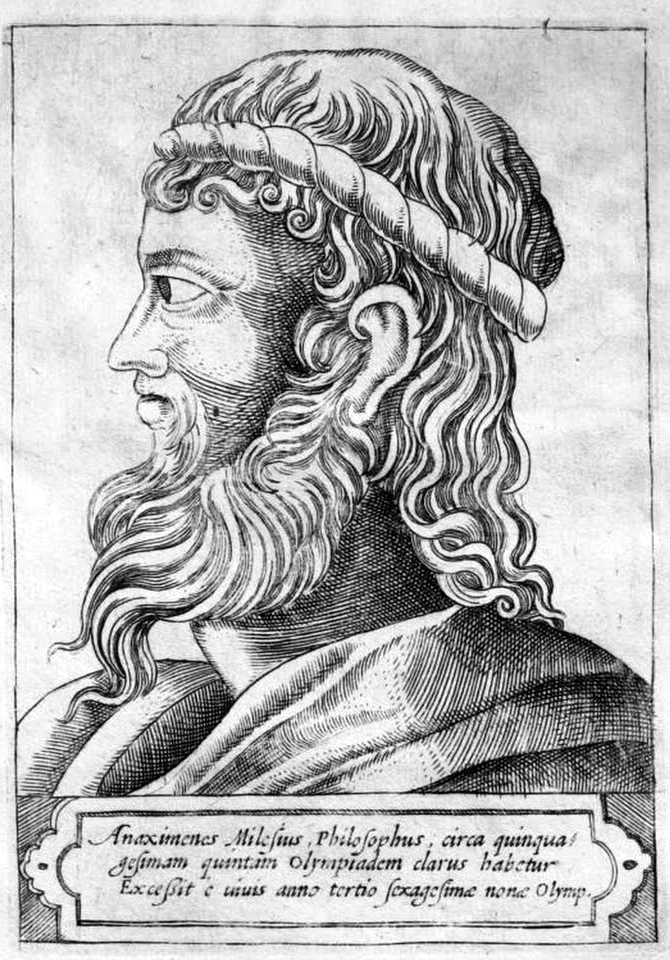
\includegraphics[width=0.5\textwidth]{../../pictures/Anaximenes_Milesius_-_Illustrium_philosophorum_et_sapientum_effigies_ab_eorum_numistatibus_extractae.png}
   \captionsetup{width=0.5\textwidth}
   \caption{\footnotesize Anaximenes of Miletus was an Ancient Greek, Pre-Socratic philosopher from Miletus in Anatolia. He was the last of the three philosophers of the Milesian School, after Thales and Anaximander. Source: \href{https://commons.wikimedia.org/wiki/File:Anaximenes_Milesius_-_Illustrium_philosophorum_et_sapientum_effigies_ab_eorum_numistatibus_extractae.png}{Wikimedia Commons}.}
   \vspace{-16pt}
\end{wrapfigure}

The genetic evolution -- that perpetual state of development which seems to affect this portion of the regions of space - has led philosophical observers to the discovery of the analogy existing among organic phenomena. As in our forests we see the same kind of tree in all the various stages of its growth, and are thus enabled to form an idea of progressive, vital development, so do we also, in the great garden of the universe, recognize the most different phases of sidereal formation. The process of condensation, which formed a part of the doctrines of Anaximenes and of the Ionian School, appears to be going on before our eyes. This subject of investigation and conjecture is especially attractive to the imagination, for in the study of the animated circles of nature, and of the action of all the moving forces of the universe, the charm that exercises the most powerful influence on the mind is derived less from a knowledge of that which is than from a perception of that which will be, even though the latter be nothing more than a new condition of a known material existence; for actual creation, of origin, the beginning of existence from non-existence, we have no experience, and can therefore form no conception.


A comparison of the various causes influencing the development manifested by the greater or less degree of condensation in the interior of nebul{\ae}, no less than a successive course of direct observations, has led to the belief that changes of form have been recognized first in Andromeda, next in the constellation Argo, and in the isolated filamentous portion of the nebula in Orion. But the want of uniformity in the power of the instruments employed, different conditions of our atmosphere, and other optical relations, render a part of the results invalid as historical evidence.

Nebulous stars must not be confounded either with irregularly shaped nebulous spots, properly so called, whose separate parts have an unequal degree of brightness (and which may, perhaps, become concentrated into stars as their circumference contracts), nor with the so-called planetary nebul{\ae}, whose circular or slightly oval disks manifest in all their parts a perfectly uniform thezres of faint light. Nebulous stars are not merely accidental bodies projected upon a nebulous ground, but are a part of the nebulous matter constituting one mass with the body which it surrounds. The not unfrequently considerable magnitude of their apparent diameter, and the remote distance from which they are revealed to us, show that both the planetary nebul{\ae} and the nebulous stars must be of enormous dimensions. New and ingenious considerations of the different influence exercised by distance\footnote{The optical considerations relative to the difference presented by a single luminous point, and by a disk subtending an appreciable angle, in which the intensity of light is constant at every distance, are explained in Arago's Analyse des Travaux de Sir William Herschel (Annuaire du Bureau des Long., 1842, p. 410-412, and 441).} on the intensity of light of a disk of appreciable diameter, and of a single self-luminous point, render it not improbable that the planetary nebul{\ae} are very remote nebulous stars, in which the difference between the central body and the surrounding nebulous covering can no longer be detected by our telescopic instruments.

The magnificent zones of the southern heavens, between $50^\circ$ and $80^\circ$, are especially rich in nebulous stars and in compressed unresolvable nebul{\ae}. The larger of the two Magellanic clouds, which circle round the starless, desert pole of the south, appears, according to the most recent researches,\footnote{The two Magellanic clouds, Nubecula major and Nubecula minor, are very remarkable objects. The larger of the two is an accumulated mass of stars, and consists of clusters of stars of irregular form, either conical masses or nebul{\ae} of different magnitudes and degrees of condensation. This is interspersed with nebulous spots, not resolvable into stars, but which are probably star dust, appearing only as a general radiance upon the telescopic field of a twenty-feet reflector, and forming a luminous ground on which other objects of striking and indescribable form are scattered. In no other portion of the heavens are so many nebulous and stellar masses thronged together in an equally small space. Nubecula minor is much less beautiful, has more unresolvable nebulous light, while the stellar masses are fewer and fainter in intensity. (From a letter of Sir John Herschel, Feldhuysen, Cape of Good Hope, 13th June, 1836.)} as a collection of clusters of stars, composed of globular clusters and nebul{\ae} of different magnitudes, and of large nebulous spots not resolvable which, producing a general brightness in the field of view, form, as it were, the background of the picture. The appearance of these clouds, of the brightly beaming constellation Argo, of the Milky Way between Scorpio, the Centaur, and the Southern Cross, the picturesque beauty, if one may so speak, of the whole expanse of the southern celestial hemisphere, has left upon my mind an ineffaceable impression. The zodiacal light, which rises in a pyramidal form, and constantly contributes, by its mild radiance, to the external beauty of the tropical nights, is either a vast nebulous ring, rotating between the Earth and Mars, or, less probably, the exterior stratum of the solar atmosphere. Besides these luminous clouds and nebul{\ae} of definite form, exact and corresponding observations indicate the existence and the general distribution of an apparently nonluminous, infinitely divided matter, which possesses a force of resistance, and manifests its presence in Encke's, and perhaps also in Biela's comet, by diminishing their eccentricity and shortening their period of revolution. Of this impeding, ethereal, and cosmical matter, it may be supposed that it is in motion; that it gravitates, notwithstanding its original tenuity; that it is condensed in the vicinity of the great mass of the Sun; and, finally, that it may, for myriads of ages, have been augmented by the vapor emanating from the tails of comets.

If we now pass from the consideration of the vaporous matter of the immeasurable regions of space (ὀυρανοῦ χóρος)\footnote{Should have made use, in the place of garden of the universe, of the beautiful expression χóρος ὀυρανοῦ, borrowed by Hesychius from an unknown poet, if χóρος had not rather signified in general an enclosed space. The connection with the German garten and the English garden, gards in Gothic (derived, according to Jacob Grimm, from gairdan, to gird), is, however, evident, as is likewise the affinity with the Slavonic grad, gorod, and as Pott remarks, in his Etymol. Forschungen, th. i., s. 144 (Etymol. Researches), with the Latin chors, whence we have the Spanish corte, the French cour, and the English word court, together with the Ossetic khart. To these may be further added the Scandinavian gard, gdrd, a place enclosed, as a court, or a country seat, and the Persian gerd, gird, a district, a circle, a princely country seat, a castle or city, as we find the term applied to the names of places in Firdusi's Schahnameh, as Siyawakschgird, Darabgird, c.

[This word is written gaard in the Danish.] -- Tr.

} -- whether, scattered without definite form and limits, it exists as a cosmical ether, or is condensed into nebulous spots, and becomes comprised among the solid agglomerated bodies of the universe, we approach a class of phenomena exclusively designated by the term of stars, or as the sidereal world.

Here, toc, we find differences existing in the solidity or density of the spheroidally agglomerated matter. Our own solar system presents all stages of mean density (or of the relation of volume to mass.) On comparing the planets from Mercury to Mars with the Sun and with Jupiter, and these two last named with the yet inferior density of Saturn, we arrive, by a descending scale to draw our illustration from terrestrial substances at the respective densities of antimony, honey, water, and pine wood. In comets, which actually constitute the most considerable portion of our solar system with respect to the number of individual forms, the concentrated part, usually termed the head, or nucleus, transmits sidereal light unimpaired. The mass of a comet probably in no case equals the five thousandth part of that of the earth, so dissimilar are the formative processes manifested in the original and perhaps still progressive agglomerations of matter. In proceeding from general to special considerations, it was particularly desirable to draw attention to this diversity, not merely as a possible, but as an actually proved fact.

\clearpage
\begin{wrapfigure}{l}{0.5\textwidth}
   \centering
   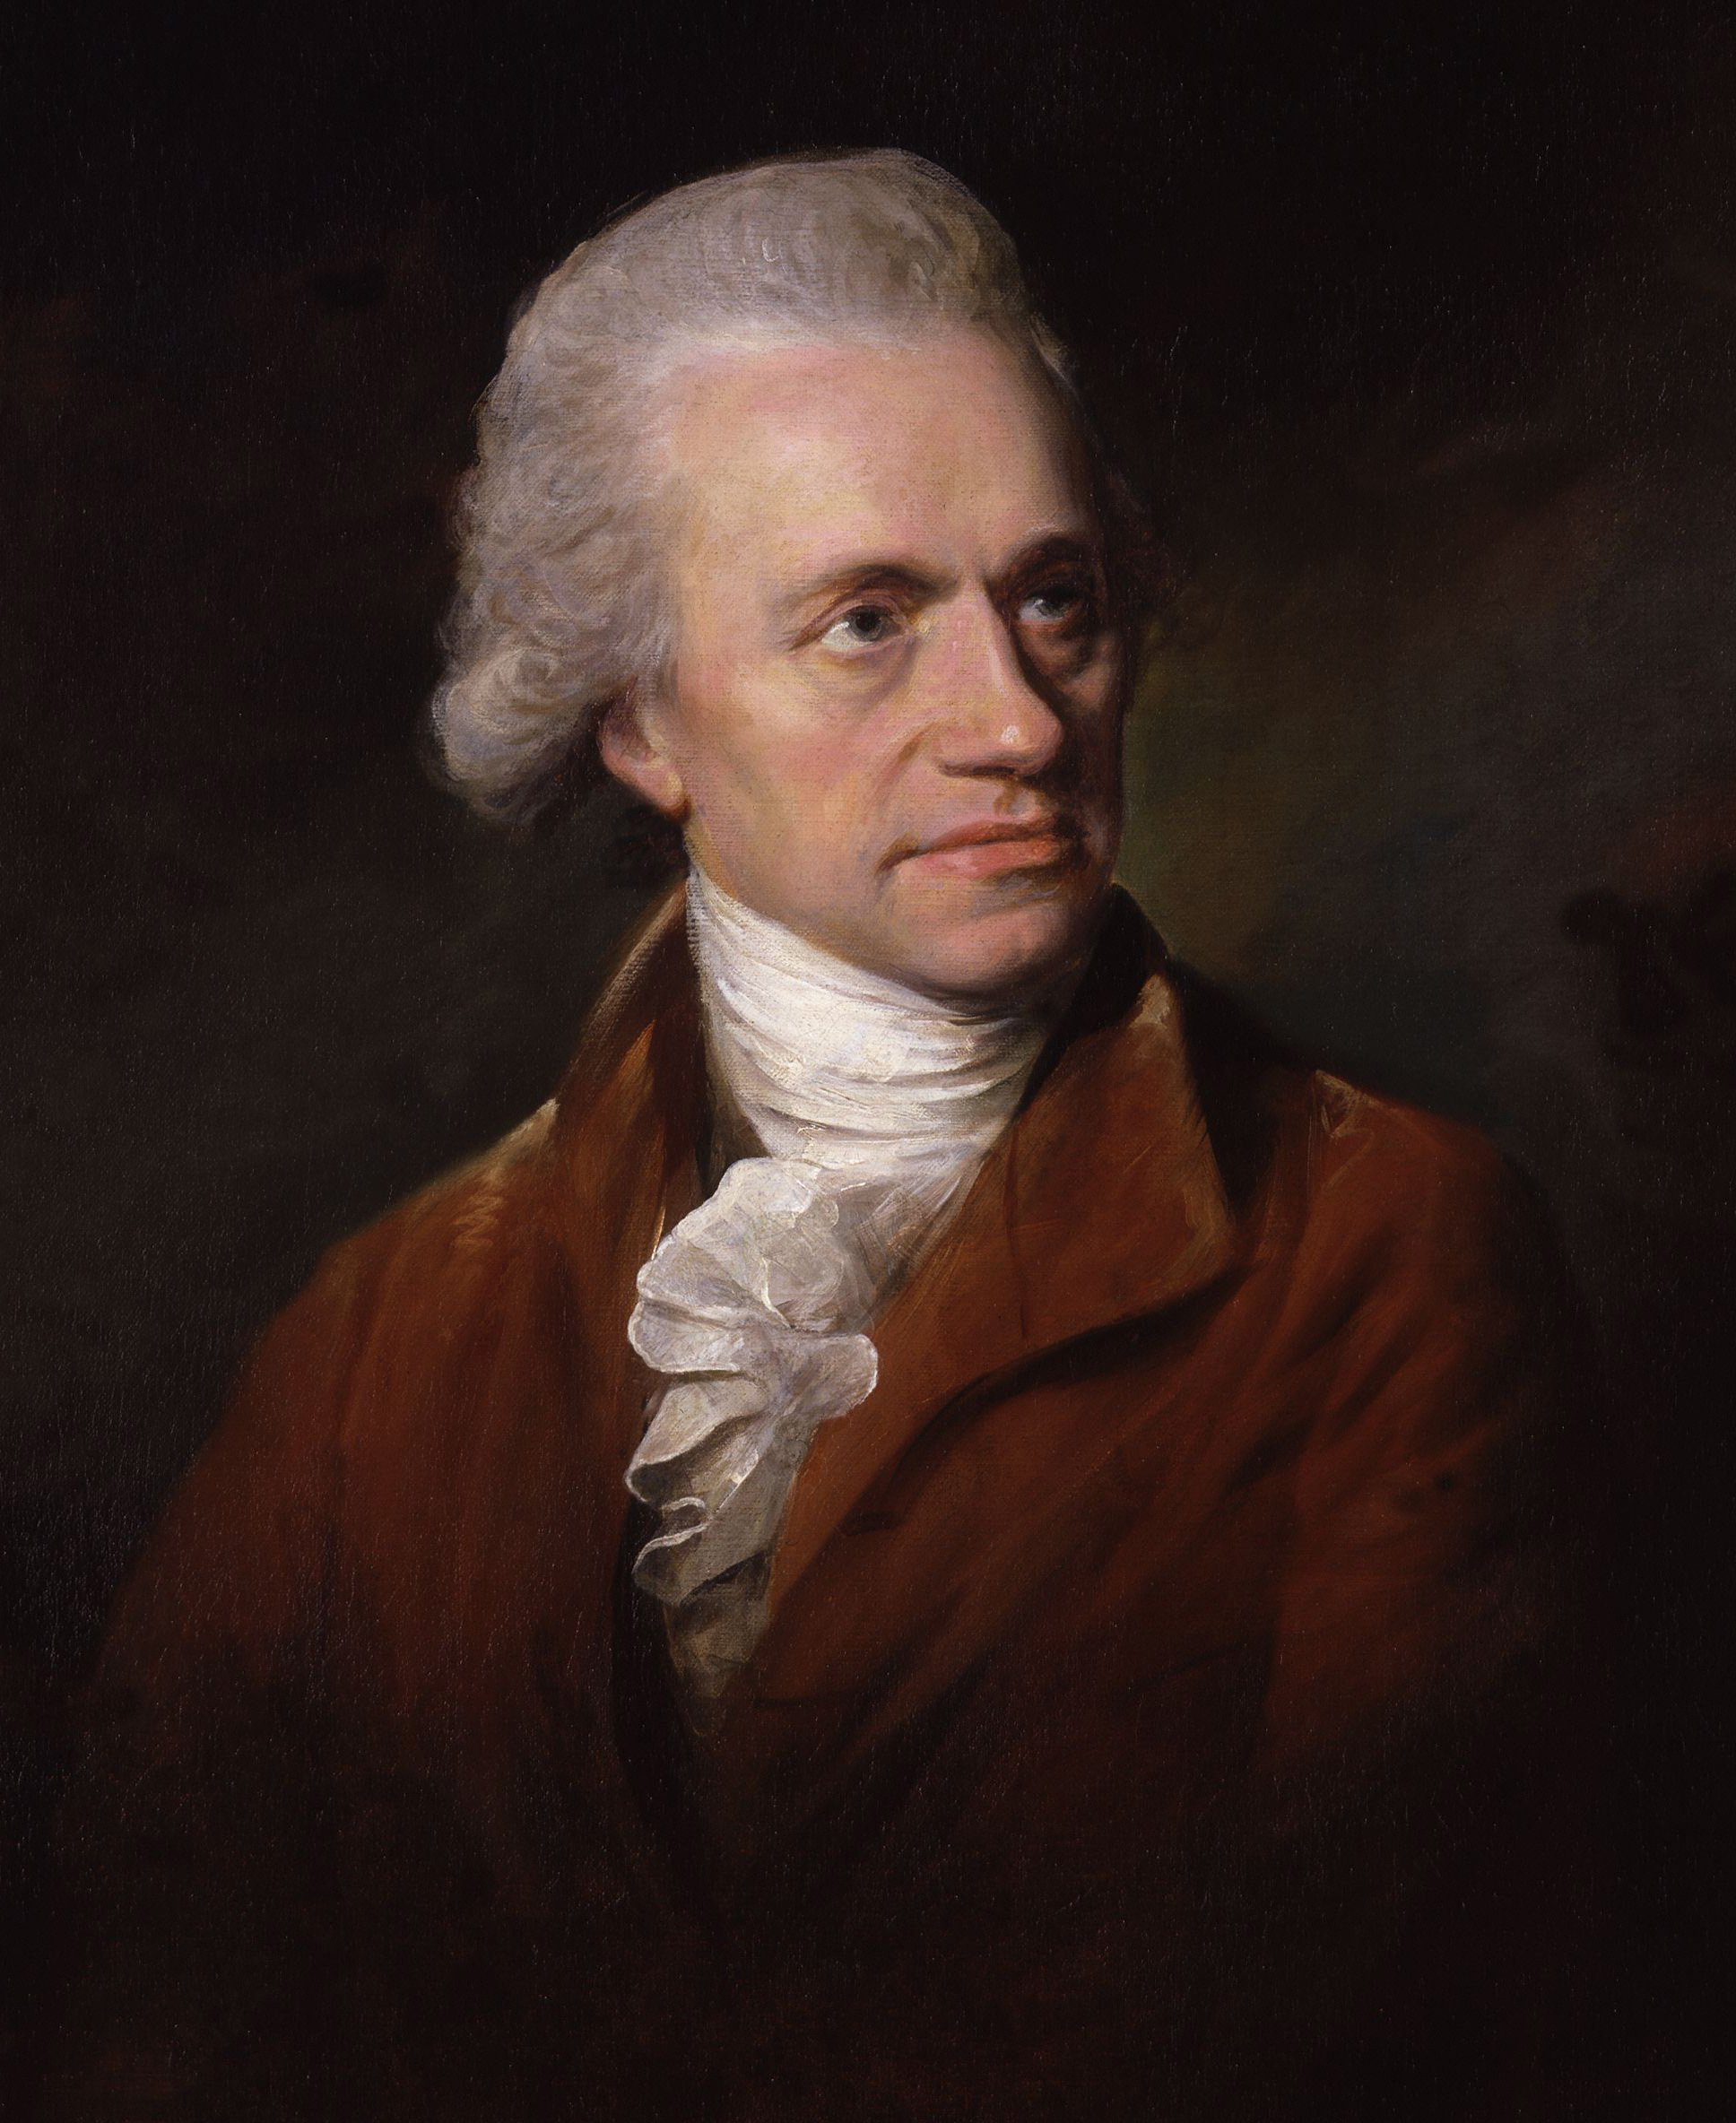
\includegraphics[width=0.5\textwidth]{../../pictures/William_Herschel01.jpg}
   \captionsetup{width=0.5\textwidth}
   \caption{\footnotesize Frederick William Herschel was a German-British astronomer and composer. Source: \href{https://commons.wikimedia.org/wiki/File:William_Herschel01.jpg}{Wikimedia Commons}.}
   \vspace{-16pt}
\end{wrapfigure}

The purely speculative conclusions arrived at by Wright, Kant, and Lambert, concerning the general structural arrangement of the universe, and of the distribution of matter in space, have been confirmed by Sir William Herschel, on the more certain path of observation and measurement. That great and enthusiastic, although cautious observer, was the first to sound the depths of heaven in order to determine the limits and form of the starry stratum which we inhabit, and he, too, was the first who ventured to throw the light of investigation upon the relations existing between the position and distance of remote nebula and our own portion of the sidereal universe. William Herschel, as is well expressed in the elegant inscription on his monument at Upton, broke through the enclosures of heaven (calorum perrupit claustra), and, like another Columbus, penetrated into an unknown ocean, from which he beheld coasts and groups of islands, whose true position it remains for future ages to determine.

Considerations regarding the different intensity of light in stars, and their relative number, that is to say, their numerical frequency on telescopic fields of equal magnitude, have led to the assumption of unequal distances and distribution in space in the strata which they compose. Such assumptions, in as far as they may lead us to draw the limits of the individual portions of the universe, cannot offer the same degree of mathematical certainty as that which may be attained in all that relates to our solar system, whether we consider the rotation of double stars with unequal velocity around one common center of gravity, or the apparent or true movements of all the heavenly bodies. If we take up the physical description of the universe from the remotest nebula, we may be inclined to compare it with the mythical portions of history. The one begins in the obscurity of antiquity, the other in that of inaccessible space; and at the point where reality seems to flee before us, imagination becomes doubly incited to draw from its own fullness, and give definite outline and permanence to the changing forms of objects.

If we compare the regions of the universe with one of the island-studded seas of our own planet, we may imagine matter to be distributed in groups, either as unresolvable nebula of different ages, condensed around one or more nuclei, or as already agglomerated into clusters of stars, or isolated spheroidal bodies. The cluster of stars, to which our cosmical island belongs, forms a lens-shaped, flattened stratum, detached on every side, whose major axis is estimated at seven or eight hundred, and its minor one at a hundred and fifty times the distance of Sirius. It would appear, on the supposition that the parallax of Sirius is not greater than that accurately determined for the brightest star in the Centaur (0''.9128), that light traverses one distance of Sirius in three years, while it also follows, from Bessel's earlier excellent Memoir\footnote{See Maclear's Results from 1839 to 1840, in the Trans. of the Astronomical Soc., vol. xii., p. 370, on a Centauri, the probable mean error being 00640. For 61 Cygni, see Bessel, in Schumacher's Jahbuch, 1839, s. 47, and Schumacher's Astron. Nachr., bd. xviii., s. 401, 402, probable mean error, 00141. With reference to the relative distances of stars of different magnitudes, how those of the third magnitude may probably be three times more remote, and the manner in which we represent to ourselves the material arrangement of the starry strata, I have found the following remarkable passage in Kepler's Epitome Astronomia Copernicane, 1618, t. i., lib. 1, p. 3439: "Solhic noster nil aliud est quam una ex fizis, nobis major et clarior visa, quia propior quam fiza. Pone terram stare ad latus, una semidiametravie lactee, tune hec via lactea apparebit circulus parvus, vel ellipsis parva, tota declinans ad latus alterum; eritque simul uno intuitu conspicua, que nune non potest nisi dimidia conspici quovis momento. Itaque fixerum sphera non tantum orbe stellarum, sed etiam cireulo lactis veraus nos deorsum est terminata.}" on the parallax of the remarkable star 61 Cygni (0''.3483), (whose considerable motion might lead to the inference of great proximity), that a period of nine years and a quarter is required for the transmission of light from this star to our planet. Our starry stratum is a disk of inconsiderable thickness, divided a third of its length into two branches; it is supposed that we are near this division, and nearer to the region of Sirius than to the constellation Aquila, almost in the middle of the stratum in the line of its thickness or minor axis.